% use option [preprint] to remove info line at bottom
% journal options: aop,aap,aos,aoas,ssy
% natbib option: authoryear
\documentclass[12pt,aoas]{imsart} %% to review
%%\documentclass[aoas]{imsart}

%%%%%%%%%%%%%%%%%%%%%%%%%%%%%%%%%%%%%%%%%%%%%%%%%%%%%%%%%%%%%%%%%%%%%%%%%%%%%%%%
% Package
\usepackage{amssymb}
\usepackage{verbatim}
%\usepackage[francais,english]{babel}
\usepackage{graphicx}
\usepackage{lineno}
\RequirePackage{natbib}
\usepackage{hyperref}
\usepackage{algorithm2e}
\RequirePackage{amsthm,amsmath}
\usepackage{color}
%\usepackage[latin1]{inputenc}
%\usepackage[table]{xcolor}

% provide arXiv number if available:
%\arxiv{arXiv:0000.0000}

% put your definitions there:
\startlocaldefs
\numberwithin{equation}{section}
\theoremstyle{plain}
\newtheorem{thm}{Theorem}[section]
\theoremstyle{definition}
\newtheorem{algo}{Algorithm}[section]
\endlocaldefs
\DeclareMathOperator*{\argmin}{arg\,min}


\begin{document}

%% To review
\baselineskip 0.8cm
\linenumbers
%%

\begin{frontmatter}

% "Title of the paper"
\title{Fast inference of individual admixture coefficients using geographic data}
\runtitle{Fast inference of individual admixture coefficients}

\begin{aug}
\author{\fnms{Kevin} \snm{Caye}\thanksref{t1}\ead[label=e1]{kevin.caye@imag.fr}},
\author{\fnms{Flora} \snm{Jay}\thanksref{t2}\ead[label=e2]{flora.jay@lri.fr}},
\author{\fnms{Olivier} \snm{Michel}\thanksref{t1}\ead[label=e3]{olivier.michel@gipsa-lab.grenoble-inp.fr}},
\and
\author{\fnms{Olivier} \snm{Fran\c cois}\thanksref{t1}
\ead[label=e4]{olivier.francois@imag.fr}}

%% \thankstext{m1}{This work has been partially supported by the LabEx PERSYVAL-Lab (ANR-11-LABX-0025-01) funded by the French program Investissement d\rq{}Avenir}
%% \thankstext{m2}{Olivier Fran\c cois acknowledges support from Grenoble INP and from the Agence Nationale de la Recherche, project AFRICROP ANR-13-BSV7-0017}
\runauthor{K. Caye et al.}

\affiliation{Universit\'e Grenoble-Alpes\thanksmark{t1} and Universit\'e Paris-Sud\thanksmark{t2}}

\address{Kevin Caye and Olivier Fran\c cois\\
Universit\'e Grenoble-Alpes\\
Centre National de la Recherche Scientifique\\ 
TIMC-IMAG UMR 5525\\
Grenoble, 38042, France\\
\printead{e1}\\
\phantom{E-mail:\ }\printead*{e4}}

\address{Flora Jay\\
Université Paris-Sud\\
Université Paris-Saclay\\
Laboratoire de Recherche en Informatique UMR 7206\\
CNRS UMR 8623\\
Orsay, 91400, France\\
\printead{e2}}

\address{Olivier Michel\\
Universit\'e Grenoble-Alpes\\
Centre National de la Recherche Scientifique\\ 
GIPSA-lab UMR 5216\\
Grenoble, 38042, France\\
\printead{e3}}


\end{aug}

% textwidth in pt: \the\textwidth \\
% textheight in pt: \the\textheight \\


\begin{abstract}
Accurately evaluating the distribution of genetic ancestry across geographic space is one of the main questions addressed by evolutionary biologists. This question has been commonly addressed through the application of Bayesian estimation programs allowing their users to estimate individual admixture proportions and allele frequencies among putative ancestral populations. Following the explosion of high-throughput sequencing technologies, several algorithms have been proposed to cope with computational burden generated by the massive data in those studies. In this context, incorporating geographic proximity in ancestry estimation algorithms is an open statistical and computational challenge. In this study, we introduce new algorithms that use geographic information to estimate ancestry proportions and ancestral genotype frequencies from population genetic data. Our algorithms combine matrix factorization methods and spatial statistics to provide estimates of ancestry matrices based on least-squares approximation.  We demonstrate the benefit of using spatial algorithms through extensive computer simulations, and we provide an example of application of our new algorithms to a set of spatially referenced samples for the plant species {\it Arabidopsis thaliana}.  Without loss of statistical accuracy, the new algorithms exhibit runtimes that are much shorter than those observed for previously developed spatial methods. Our algorithms are implemented in the {\tt R} package, {\tt tess3r}, which is available from \url{https://github.com/BioShock38/TESS3_encho_sen}. 
\end{abstract}

\begin{keyword}
\kwd{Ancestry Estimation Algorithms}
\kwd{Genotypic Data}
\kwd{Geographic Data}
\kwd{Fast Algorithms}
\end{keyword}

\end{frontmatter}


\section{Introduction}

High-throughput sequencing technologies have enabled studies of genetic ancestry
for model and non-model species at an unprecedented pace. In this context,
ancestry estimation algorithms are important for demographic analysis, medical
genetics including genome-wide association studies, conservation and landscape
genetics~\citep{Pritchard2000, Tang2005, Schraiber2015, Segelbacher2010,
  Francois2015}. With increasingly large data sets, Bayesian approaches to the
inference of population structure, exemplified by the computer program {\tt
  structure} \citep{Pritchard2000}, have been replaced by approximate algorithms
that run several orders faster than the original version~\citep{Tang2005,
  Alexander2011, Frichot2014, Raj2014}. Considering $K$ ancestral populations or
genetic clusters, those algorithms estimate ancestry coefficients following two
main directions: model-based and model-free approaches. In model-based
approaches, a likelihood function is defined for the matrix of ancestry
coefficients, and estimation is performed by maximizing the log-likelihood
function. For {\tt structure} and related models, model assumptions include
linkage equilibrium and Hardy-Weinberg equilibrium in ancestral populations. The
first approximation to the original algorithm was based on an
expectation-minimization algorithm~\citep{Tang2005}, and more recent likelihood
algorithms are implemented in the programs {\tt admixture} and {\tt
  faststructure} \citep{Alexander2011, Raj2014}. In model-free approaches,
ancestry coefficients are estimated by using least-squares methods or factor
analysis. Model-free methods make no assumptions about the biological processes
that have generated the data. To estimate ancestry matrices,
\cite{Engelhardt2010} proposed to use sparse factor analysis, \cite{Frichot2014}
used sparse non-negative matrix factorization algorithms, and \cite{Popescu2014}
used kernel-principal component analysis. Least-squares methods accurately
reproduce the results of likelihood approaches under the model assumptions of
those methods. In addition, model-free methods provide approaches that are valid
when the assumptions of likelihood approaches are not met~\citep{Frichot2014}.
Model-free methods are generally faster than model-based methods.
   
Among model-based approaches to ancestry estimation, an important class of
methods have improved the Bayesian model of {\tt structure} by incorporating
geographic data through spatially informative prior
distributions~\citep{Chen2007, Corander2008}. Under isolation-by-distance
patterns~\citep{Wright1943, Malecot1948}, spatial algorithms provide more robust
estimates of population structure than non-spatial algorithms which can lead to
biased estimates of the number of clusters~\citep{Durand2009}. Some Bayesian
methods are based on Markov chain Monte Carlo algorithms which are
computer-intensive~\citep{Francois2010}. Recent efforts to improve the inference
of ancestral relationships in a geographical context have mainly focused on the
localization of recent ancestors~\citep{Baran2013, Lao2014, Yang2014,
  bhaskar2016, ranola2014}. In these applications, spatial information is used
in a predictive framework that assigns ancestors to putative geographic origins.
While fast geographic estimation of individual ancestry proportions has been
proposed previously~\citep{Caye2016, bradburd2016}, there is a growing need to
develop individual ancestry estimation algorithms that reduce computational cost
in a geographically explicit framework.

 In this study, we present two new algorithms for the estimation of ancestry
 matrices based on geographic and genetic data. The new algorithms solve a least
 squares optimization problem as defined by~\cite{Caye2016}, based on
 Alternating Quadratic Programming (AQP) and Alternating Projected Least Squares
 (APLS). While AQP algorithms have a well-established theoretical
 background~\citep{Bertsekas1995}, this is not the case of APLS algorithms.
 Using coalescent simulations, we provide evidence that the estimates computed
 by APLS algorithms are good approximations to the solutions of AQP algorithms.
 In addition, we show that the performances of APLS algorithms scale to the
 dimensions of modern data sets. We discuss the application of our algorithms to
 data from European ecotypes of {\it Arabidopsis thaliana}, for which individual
 genomic a geographic data are available~\citep{Horton2012}.




\clearpage
\newpage

\section{New methods}

%% Présenter le problème et la factorisation matricielle
%%
%%

In this section we present two new algorithms for estimating individual
admixture coefficients and ancestral genotype frequencies assuming $K$ ancestral
populations. In addition to genotypes, the new algorithms require individual
geographic coordinates of sampled individuals.

\paragraph{$Q$ and $G$-matrices} Consider a genotypic matrix, {\bf Y}, recording
data for $n$ individuals at $L$ polymorphic loci for a $p$-ploid species (common
values for $p$ are $p = 1,2$). For autosomal SNPs in a diploid organism, the
genotype at locus $\ell$ is an integer number, 0, 1 or 2, corresponding to the
number of reference alleles at this locus. In our algorithms, disjunctive forms
are used to encode each genotypic value as the indicator of a heterozygote or a
homozygote locus (Frichot et al. 2014). For a diploid organism each genotypic
value $,0,1,2$ is encoded as $100$, $010$ and $001$. For $p$-ploid organisms,
there are $(p+1)$ possible genotypic values at each locus, and each value
corresponds to a unique disjunctive form. While our focus is on SNPs, the
algorithms presented in this section extend to multi-allelic loci without loss
of generality. Moreover, the method can be easily extended to genotype
likelihoods by using the likelihood to encode each genotypic
value~\citep{Korneliussen2014}.

Our algorithms provide statistical estimates for the matrix ${\bf Q} \in
\mathbb{R}^{K \times n}$ which contains the admixture coefficients, ${\bf
  Q}_{i,k}$, for each sampled individual, $i$, and each ancestral population,
$k$. The algorithms also provide estimates for the matrix ${\bf G} \in
\mathbb{R}^{(p+1)L \times K}$, for which the entries, ${\bf G}_{(p+1)\ell + j,
  k}$, correspond to the frequency of genotype $j$ at locus $\ell$ in population
$k$. Obviously, the $Q$ and $G$-matrices must satisfy the following set of
probabilistic constraints

$$
\quad {\bf Q},{\bf G} \geq 0 \, , \quad \sum_{k=1}^K {\bf Q}_{i,k} = 1 \, ,
\quad \sum_{j=0}^p {\bf G}_{(p+1)\ell + j, k} = 1 \, , \quad j = 0,1,\dots, p,
$$
for all $i, k$ and $\ell$. Using disjunctive forms and the law of total
probability, estimates of {\bf Q} and {\bf G} can be obtained by factorizing the
genotypic matrix as follows ${\bf Y}$=${\bf Q}\,{\bf G}^T$~\citep{Frichot2014}.
Thus the inference problem can be solved by using constrained nonnegative matrix
factorization methods~\citep{Lee1999, Cichocki2009}. In the sequel, we shall use
the notations $\Delta_Q$ and $\Delta_G$ to represent the sets of probabilistic
constraints put on the {\bf Q} and {\bf G} matrices respectively.


\paragraph{Geographic weighting} Geography is introduced in the matrix
factorization problem by using weights for each pair of sampled individuals. The
weights impose regularity constraints on ancestry estimates over geographic
space. The definition of geographic weights is based on the spatial coordinates
of the sampling sites, $(x_i)$. Samples close to each other are given more
weight than samples that are far apart. The computation of the weights starts
with building a complete graph from the sampling sites. Then the weight matrix
is defined as follows

$$
w_{ij} = \exp( - {\rm dist}( x_i, x_j )^2/ \sigma^2),
$$
\noindent where dist$( x_i, x_j )$ denotes the geodesic distance between sites
$x_i$ and $x_j$, and $\sigma$ is a range parameter.


Next, we introduce the {\it Laplacian matrix} associated with the geographic
weight matrix, {\bf W}. The Laplacian matrix is defined as ${\bf \Lambda}$ =
{\bf D} $-$ {\bf W} where {\bf D} is a diagonal matrix with entries ${\bf
  D}_{i,i} = \sum_{j = 1}^n {\bf W}_{i,j}$, for $i = 1, \dots,
n$~\citep{Belkin2003}. Elementary matrix algebra shows that~\citep{DengCai2011}

$$
 {\rm Tr} ({\bf Q}^T {\bf \Lambda} {\bf Q})  = \frac12 \sum_{i,j = 1}^n  w_{ij}  \|   {\bf Q}_{i,.}  - {\bf Q}_{j,.} \|^2 \, .
$$
In our approach, assuming that geographically close individuals are more likely to share ancestry than individuals at distant sites is thus equivalent to minimizing the quadratic form ${\cal C}({\bf Q}) ={\rm Tr} ({\bf Q}^T {\bf \Lambda} {\bf Q})$ while estimating the matrix ${\bf Q}$. 

\paragraph{Least-squares optimization problems} Estimating the matrices ${\bf
  Q}$ and ${\bf G }$ from the observed genotypic matrix ${\bf Y}$ is performed
through solving an optimization problem defined as follows~\citep{Caye2016}

\begin{equation}
\begin{aligned}
& \underset{Q, G}{\text{min}}
& & {\rm LS}({\bf Q}, {\bf G}) =   \|  {\bf Y} - {\bf QG}^T \|^2_{\rm F} +  \alpha {\cal C}({\bf Q}) , \\
& \text{s.t.} & &  {\bf Q} \in \Delta_Q , \\
& & &  {\bf G} \in \Delta_G . \\
\end{aligned}
\label{eq:LS}
\end{equation}
\noindent The notation $\| {\bf M} \|_{\rm F}$ denotes the Frobenius norm of a
matrix, {\bf M}. The regularization parameter $\alpha $ controls the regularity
of ancestry estimates over geographic space. Large values of $\alpha $ imply
that ancestry coefficients have similar values for nearby individuals, whereas
small values ignore spatial autocorrelation in observed allele frequencies.

\paragraph{The Alternating Quadratic Programming (AQP) method} Because the
poly\-edrons $\Delta_Q$ and $\Delta_G$ are convex sets and the LS function is
convex with respect to each variable ${\bf Q}$ or ${\bf G}$ when the other one
is fixed, the problem~\eqref{eq:LS} is amenable to the application of block
coordinate descent~\citep{Bertsekas1995}. The APQ algorithm starts from initial
values for the $G$ and $Q$-matrices, and alternates two steps. The first step
computes the matrix {\bf G} while {\bf Q} is kept fixed, and the second step
permutates the roles of {\bf G} and {\bf Q}. Let us assume that {\bf Q} is fixed
and write {\bf G} in a vectorial form, $g = {\rm vec({\bf G})} \in
\mathbb{R}^{K(p + 1)L}$. The first step of the algorithm actually solves the
quadratic programming subproblem, 

\begin{equation}
\begin{aligned}
g^\star = \underset{g \in \Delta_G}{\arg \min}  ( -2  v^T_Q \, g + g^T {\bf D}_Q g ) \, ,  
\end{aligned}
\label{eq:AQPg}
\end{equation}
\noindent where ${\bf D}_Q = {\bf I}_{(p+1)L} \otimes {\bf Q}^T {\bf Q}$ and
$v_Q = {\rm vec}({\bf Q}^T {\bf Y})$. Here, $\otimes$ denotes the Kronecker
product and ${\bf I}_d$ is the identity matrix with $d$ dimensions. The block
structure of the matrix ${\bf D}_Q$ allows us to decompose the
subproblem~\eqref{eq:AQPg} into $L$ independent quadratic programming problems
with $K(p + 1)$ variables. Now, consider that {\bf G} is the value obtained
after the first step of the algorithm, and write {\bf Q} in a vectorial form, $q
= {\rm vec({\bf Q})} \in \mathbb{R}^{nK}$. The second step solves the following
quadratic programming subproblem. Find

\begin{equation}
\begin{aligned}
q^\star = \underset{q \in \Delta_Q}{\arg \min} ( -2 v^T_G \, q + q^T {\bf D}_G q ) \,  ,
\end{aligned}
\label{eq:AQPq}
\end{equation}
\noindent where ${\bf D}_G = {\bf I}_{n} \otimes {\bf G}^T {\bf G } + \alpha
{\bf \Lambda} \otimes {\bf I}_K$ and $v_G = {\rm vec}({\bf G}^T{\bf Y}^T)$.
Unlike subproblem~\eqref{eq:AQPg}, subproblem~\eqref{eq:AQPq} can not be
decomposed into smaller problems. Thus, the computation of the second step of
the AQP algorithm implies to solve a quadratic programming problem with $nK$
variables which can be problematic for large samples ($n$ is the sample size).
The AQP algorithm is described in details in Appendix~\ref{algo:aqp}. For AQP,
we have the following convergence result.
\begin{thm}
\label{th}
	The AQP algorithm converges to a critical point of problem~\eqref{eq:LS}.
\end{thm}
\begin{proof}
  The quadratic convex functions defined in subproblems~\eqref{eq:AQPg}
  and~\eqref{eq:AQPq} have finite lower bounds. The convex sets $\Delta_Q$ and
  $\Delta_G$ are compact non-empty sets. Thus the sequence generated by the AQP
  algorithm is well-defined, and has limit points. According to Corollary 2 of
  ~\cite{Grippo2000}, we conclude that the AQP algorithm converges to a critical
  point of problem~\eqref{eq:LS}.
\end{proof}

\paragraph{Alternating Projected Least-Squares (APLS)} In this paragraph, we
introduce an APLS estimation algorithm which approximates the solution of
problem~\eqref{eq:LS}, and reduces the complexity of the AQP algorithm. The APLS
algorithm starts from initial values of the $G$ and $Q$-matrices, and alternates
two steps. The matrix {\bf G} is computed while {\bf Q} is kept fixed, and {\it
  vice versa}. Assume that the matrix {\bf Q} is known. The first step of the
APLS algorithm solves the following optimization problem. Find

\begin{equation}
{\bf G}^\star = \arg \min  \|  {\bf Y} - {\bf QG}^T \|^2_{\rm F} \, .
\end{equation}
This operation can be done by considering $(p+1)L$ (the number of columns of
${\bf Y}$) independent optimization problems running in parallel. The operation
is followed by a projection of ${\bf G}^\star$ on the polyedron of constraints,
$\Delta_G$. For the second step, assume that {\bf G} is set to the value
obtained after the first step is completed. We compute the eigenvectors, {\bf
  U}, of the Laplacian matrix, and we define the diagonal matrix ${\bf \Delta}$
formed by the eigenvalues of ${\bf \Lambda}$ (The eigenvalues of ${\bf \Lambda}$
are non-negative real numbers). According to the spectral theorem, we have

$$
{\bf \Lambda} = {\bf U}^T {\bf \Delta} {\bf U} \, .
$$
\noindent  After this operation, we project the data matrix {\bf Y} on the basis of eigenvectors as follows

$$
{\rm proj} ({\bf Y}) = {\bf U}{\bf Y} \, , 
$$
\noindent and, for each individual, we solve the following optimization problem

\begin{equation}
q_i^\star = \arg \min  \|  {\rm proj} ({\bf Y})_i  - {\bf G} q \|^2 + \alpha \lambda_i \| q \|^2  \, ,
\label{eq:APSLq}
\end{equation}
\noindent where proj({\bf Y}$)_i$ is the $i$th row of the projected data matrix,
proj({\bf Y}), and $\lambda_i$ is the $i$th eigenvalue of ${\bf \Lambda}$. The
solutions, $q_i$, are then concatenated into a matrix, ${\rm conc}(q)$, and
${\bf Q}$ is defined as the projection of the matrix ${\bf U}^T {\rm conc}(q)$
on the polyedron $\Delta_Q$. The complexity of step~\eqref{eq:APSLq} grows
linearly with $n$, the number of individuals. While the theoretical convergence
properties of AQP algorithms are lost for APLS algorithms, the APLS algorithms
are expected to be good approximations of AQP algorithms. The APLS algorithm is
described in details in Appendix~\ref{algo:apls}.


\paragraph{Choice of hyper-parameters.} In ancestry estimation programs, a
number of practices have evolved in order to set the model hyper-parameters.

Those practices rely on heuristics or empirical rules for determining the prior
parameters. For example, the program structure implements weakly informative
prior distributions for ancestry proportions~\citep{wang2017}, the program {\tt
  admixture} has a set of regularization parameters that encourages shrinkage
and “aggressive” parsimony on ancestry estimates~\citep{Alexander2011}, and so
does the Bayesian version TESS 2.3~\citep{Durand2009}. Choosing the number of
ancestral populations is based on cross-validation methods or information
theoretic measures. Our model has three hyper-parameters: the number of factors,
$K$, the penalty constant, $\alpha$, and the range parameter, $\sigma$.
Determining those constants is notoriously difficult and can be costly in
applications. In order to reduce the computational burden, the hyper-parameters
$\alpha$ and $\sigma$ are set as user-defined options. This option allows an
advanced user to explore different values with cross-validation or with her own
heuristics. Less advanced users could use the default values of the
hyper-parameters evaluated in our simulation study.
 

\paragraph{Range parameter.} Testing correlations between genetic and geographic
has a long tradition in population genetics. Popular approaches are based on
Mantel tests~\citep{mantel1967} and spatial autocorrelation
measures~\citep{hardy1999, epperson1996}. Prior to the application of our spatial ancestry
estimation program, we investigated biologically relevant values for the range
parameter by using spatial variograms~\citep{Cressie1993}. The variogram was
extended to genotypic data as follows


\begin{equation}
\gamma(h) = \frac{1}{2 |N(h)|} \sum_{i,j \in N(h)} \frac{1}{L} \sum_{l = 1}^{(p+1)L} |Y_{i,l} - Y_{j,l}|,
\label{eq:gamma}
\end{equation}
where $N(h)$ is defined as the set of individuals separated by geographic
distance $h$. Visualizing the variogram provides useful information on the level
of spatial autocorrelation in the data, and yields empirical estimates of the
range parameter. More naïve estimates such as an average geodesic distance
computed over a fraction of neighboring sites in the sample also performed well
in simulations, and they are also proposed to the program users.

\paragraph{Regularization parameter.} A default value for the regularization
parameter $\alpha$ was set so that the weights for the loss function and for
the penalty term ${\cal C}({\bf Q})$ are of similar order. We proposed to divide
each term by its maximum value. This amount to consider $\alpha$ equal to $L /
\lambda_\max$, where $\lambda_\max$ is the largest eigenvalue of the Laplacian
matrix (The Laplacian matrix has nonnegative eigenvalues).

\paragraph{Number of factors.} The number of ancestral populations, $K$, can be
evaluated by using a cross-validation technique based on imputation of masked
genotypes~\citep{wold1978,eastment1982, Alexander2011, Frichot2014}. The
cross-validation procedure partitions the genotypic matrix entries into a
learning set and a test set in which 5\% of all genotypes are tagged as masked
entries. The genotype probabilities for the masked entries are predicted from
the factor estimates obtained from unmasked entries. Then, a cross-entropy
between the predicted and truly observed genotype frequencies is computed, and
smaller values of that criterion indicate better choices.

\paragraph{Comparison with {\tt tess3}} The algorithm implemented in a previous
version of {\tt tess3} also provides another approximation of the solution
of problem~\eqref{eq:LS}. The {\tt tess3} algorithm first computes a Cholesky
decomposition of the Laplacian matrix. Then, by a change of variables, the
least-squares problem is transformed into a sparse nonnegative matrix
factorization problem~\citep{Caye2016}. Solving the sparse non-negative matrix
factorization problem relies on the application of existing
methods~\citep{Kim2011, Frichot2014}. The methods implemented in {\tt tess3}
have an algorithmic complexity that increases linearly with the number of loci
and the number of clusters. They lead to estimates that accurately reproduce
those of the Monte Carlo algorithms implemented in the Bayesian method {\tt
  tess} 2.3~\citep{Caye2016}. Like for the AQP method, the {\tt tess3} previous
algorithms have an algorithmic complexity that increases quadratically with the
sample size.




\paragraph{Ancestral population differentiation statistics and local adaptation
  scans} Assuming $K$ ancestral populations, the $Q$ and $G$-matrices obtained
from the AQP and from the APLS algorithms were used to compute single-locus
estimates of a population differentiation statistic similar to $F_{\rm
  ST}$, as follows

$$
F^{Q}_{\rm ST} = 1 - \sum_{k=1}^K  q_k \frac{f_k (1-f_k)}{f(1-f)} \, ,
$$
\noindent where $q_k$ is the average of ancestry coefficients over sampled
individuals, $q_k = \sum_{i =1}^n Q_{i,k}/n$, for the cluster $k$, $f_k$ is the
ancestral allele frequency in population $k$ at the locus of interest,

$$
f_k =  \sum_{j = 1}^p  j G_{(p+1)(\ell) + j, k}/p ,
$$
and $f = \sum_{k = 1}^K q_k f_k$~\citep{Martins2016}.
For a particular locus, the formula for $F^Q_{\rm ST}$ corresponds to the
proportion of the genetic variation (or variance) in ancestral allele frequency
that can be explained by latent population structure

$$
F^Q _{\rm ST}  =  \frac{\sigma^2_T - \sigma^2_S}{\sigma^2_T },
$$
where $\sigma^2_T$ is the total variance and $\sigma^2_S$ is the error
variance~\citep{weir1996}. Following ANOVA theory, the $F^Q_{\rm ST}$ statistics
were used to perform statistical tests of neutrality at each locus, by comparing
the observed values to their expectations from the genome-wide background. The
test was based on the squared $z$-score statistic, $z^2 = (n-K) F^{Q}_{\rm
  ST}/(1 - F^{Q}_{\rm ST})$, for which a chi-squared distribution with $K-1$
degrees of freedom was assumed under the null-hypothesis. To avoid an increased
number of false positive tests, we adopted an empirical null-hypothesis testing
approach that recalibrates the null-hypothesis for the background levels of
population differentiation expected at selectively neutral SNPs~\citep{efron2004}.
The calibration of the null-hypothesis was achieved by using genomic control to
adjust the test statistics~\citep{Devlin1999, Francois2016}. After recalibration
of the null-hypothesis, the control of the false discovery rate was achieved by
using the Benjamini-Hochberg algorithm~\citep{Benjamini1995}.


\paragraph{{\tt R} package} We implemented the AQP and APLS algorithms and
improved graphical tools in the {\tt R} package {\tt tess3r}, available from
Github and submitted to the Comprehensive R Archive Network (R Core Team, 2016).


\section{Simulated and real data sets}
\paragraph{Coalescent simulations} We used the computer program {\tt ms} to
perform coalescent simulations of neutral and outlier SNPs under spatial models
of admixture~\citep{Hudson2002}. Two ancestral populations were created from the
simulation of Wright\rq{}s two-island models. The simulated data sets contained
admixed genotypes for $n$ individuals for which the admixture proportions varied
continuously along a longitudinal gradient~\citep{Durand2009, Francois2010}. In
those scenarios, individuals at each extreme of the geographic range were
representative of their population of origin, while individuals at the center of
the range shared intermediate levels of ancestry in the two ancestral
populations~\citep{Caye2016}. For those simulations, the $Q$ matrix, ${\bf
  Q}_0$, was entirely described by the location of the sampled individuals.


Neutrally evolving ancestral chromosomal segments were generated by simulating
DNA sequences with an effective population size $N_0 = 10^6$ for each ancestral
population. The mutation rate per bp and generation was set to $\mu = 0.25
\times 10^{-7}$, the recombination rate per generation was set to $r = 0.25
\times 10^{-8}$, and the parameter $m$ was set to obtained neutral levels of
$F_{\rm ST}$ ranging between values of $0.005$ and $0.10$. The number of base
pairs for each DNA sequence was varied between 10k to 300k to obtain numbers of
polymorphic loci ranging between 1k and 200k after filtering out SNPs with
minor allele frequency lower than 5$\%$. To create SNPs with values in the tail
of the empirical distribution of $F_{\rm ST}$, additional ancestral chromosomal
segments were generated by simulating DNA sequences with a migration rate $m_s$
lower than $m$. The simulations reproduced the reduced levels of diversity and
the increased levels of differentiation expected under hard selective sweeps
occurring at one particular chromosomal segment in ancestral
populations~\citep{Martins2016}. For each simulation, the sample size was varied
in the range $n =$ 50-700.

We compared the AQP and APLS algorithm estimates with those obtained with the
{\tt tess3} algorithm. Each program was run 5 times on the same simulated data.
Using $K = 2$ ancestral populations, we computed the root mean squared error
(RMSE) between the estimated and known values of the $Q$-matrix, and between the
estimated and known values of the $G$-matrix. To evaluate the benefit of spatial
algorithms, we compared the statistical errors of APLS algorithms to the errors
obtained with {\tt snmf} method that reproduces the outputs of the {\tt
  structure} program accurately~\citep{Frichot2014,Frichot2015}. To quantify the
performances of neutrality tests as a function of ancestral and observed levels
of $F_{\rm ST}$, we used the area under the precision-recall curve (AUC) for
several values of the selection rate. Subsamples from a real data set were used
to perform a runtime analysis of the AQP and APLS algorithms ({\it A. thaliana}
data, see below). Runtimes were evaluated by using a single computer processor
unit Intel Xeon 2.0 GHz.

\paragraph{Application to human data.} To evaluate the robustness of our
approach to a situation where admixture was the consequence of large
displacement rather than contact between proximal populations, we studied the
case of African-American populations. This is an interesting case for which the
incorporation of geographic data could potentially bias estimation of ancestry
coefficients. Genotypes with minor allele frequency greater than $5 \%$ were
obtained from a public release of the
% TODO number of snips + number of infiv by pop
1000 Genomes project phase 3 for African Americans (ASW,
?? individuals), Africans (YRI from Nigeria and LWK from Kenya, ?? individuals),
and Europeans (GBR from the United Kingdom and
TSI from Italy, ?? individuals)~\citep{1000genome}. A total of ?? SNPs were analyzed with geographic data
corresponding to the country of origin of individual samples. We compared the
estimates from the APLS algorithm applied with its default parameter settings to
the results of the {\tt snmf} program that do not make use of geographic information.

\paragraph{Application to European ecotypes of {\it Arabidopsis thaliana}} We
used the APLS algorithm to survey spatial population genetic structure and to
investigate the molecular basis of adaptation by considering 214k SNPs from
1,095 European ecotypes of the plant species {\it A. thaliana}
~\citep{Horton2012}. The cross-validation criterion was used to evaluate the
number of clusters in the sample, and a statistical analysis was performed to
evaluate the range of the variogram from the data. We used {\tt R} functions of
the {\tt tess3r} package to display interpolated admixture coefficients on a
geographic map of Europe (R Core team 2016). A gene ontology enrichment analysis
using the software AMIGO~\citep{Carbon2009} was performed in order to evaluate
which molecular functions and biological processes might be involved in local
adaptation of {\it A. thaliana} in Europe.



\clearpage
\newpage


\section{Results}
\paragraph{Statistical errors} We used coalescent simulations of neutral
polymorphisms under spatial models of admixture to compare the statistical
errors of the AQP and APLS estimates with those of the {\tt tess3}
algorithm~\citep{Caye2016}. The ground truth for the $Q$-matrix (${\bf Q}_0$)
was computed from the mathematical model for admixture proportions used to
generate the data. For the $G$-matrix, the ground truth matrix (${\bf G}_0$) was
computed from the empirical genotype frequencies in the two population samples
before an admixture event. The root mean squared errors (RMSE) for the ${\bf Q}$
and ${\bf G}$ estimates decreased as the sample size and the number of loci
increased (Figure~\ref{fig:fig1}). For all algorithms, the statistical errors were generally
small when the number of loci was greater than $10$k SNPs. Those results
provided evidence that the three algorithms produced equivalent estimates of the
matrices ${\bf Q}_0$ and ${\bf G}_0$. The results also provided a check
that the APLS and {\tt tess3} algorithms converged to the same estimates as
those obtained after the application of the AQP algorithm, which is guaranteed
to converge mathematically.


\paragraph{The benefit of including spatial information in algorithms} Using
neutral coalescent simulations of spatial admixture, we compared the statistical
estimates obtained from a spatial algorithm (APLS) and a non-spatial algorithm
(sNMF, Frichot et al. 2014). For various levels of ancestral population
differentiation, estimates obtained from the spatial algorithm were more
accurate than for those obtained using non-spatial approaches (Figure~\ref{fig:fig2}). For
the larger samples, much finer population structure was detected with the
spatial method than with the non-spatial algorithm (Figure~\ref{fig:fig2}).

In simulations of outlier loci, we used the area under the precision-recall
curve (AUC) for quantifying the performances of tests based on the estimates of
ancestry matrices, {\bf Q} and {\bf G}. In addition, we computed AUCs for
$F_{\rm ST}$-based neutrality tests using truly ancestral genotypes. As they
represented the maximum reachable values, AUCs based on truly ancestral
genotypes were always higher than those obtained for tests based on
reconstructed matrices. For all values of the relative selection intensity, AUCs
were higher for spatial methods than for non-spatial methods (Figure~\ref{fig:fig3}, the
relative selection intensity is the ratio of migration rates at neutral and
adaptive loci). For high selection intensities, the performances of tests based
on estimates of ancestry matrices were close to the optimal values reached by
tests based on true ancestral frequencies. These results provided evidence that
including spatial information in ancestry estimation algorithms improves the
detection of signatures of hard selective sweeps having occurred in unknown
ancestral populations.

\paragraph{Sensitivity of estimates to spatial measurements.} Next, we used the
simulated data sets to evaluate the robustness of APLS estimates to inaccurate
measurements of spatial coordinates. To this aim, Gaussian noise was added to
truly observed geographic coordinates by considering values of the
noise-to-signal ratio ranging from 0 to 3. We computed variograms in all
cases, and found that the spatial signal was removed from simulations with a
noise-to-signal ratio of ??? ($\sigma \approx 0$), while the signal was still
observable with a noise-to-signal ratio of 1.
%% TODO paragraph quand fig OK
A noise-to-signal ratio of 1 increased statistical errors in the $Q$-matrix
estimates, but the RMSEs remained generally lower than for methods without
spatial coordinates ($\alpha = 0$ and sNMF, Figure~\ref{fig:fig2_5}). For a noise-to-signal ratio
of 3, errors were higher than for methods without spatial coordinates
(Figure~\ref{fig:fig2_5}). To a large extent, estimates from the APLS algorithm
were robust to uncertainty in spatial measurements. Standard graphical tests
such as a variogram analysis can help deciding whether our spatially explicit
algorithm is useful or not.


\paragraph{Runtime and convergence analyses} We subsampled a large SNP data set
for {\it A. thaliana} ecotypes to compare the convergence properties and
runtimes of the {\tt tess3}, AQP, and APLS algorithms. In those experiments, we
used $K = 6$ ancestral populations, and replicated 5 runs for each simulation.
For $n = 100-600$ individuals ($L = 50$k SNPs), the APLS algorithm required more
iterations (25 iterations) than the AQP algorithm (20 iterations) to converge to
its solution (Figure~\ref{fig:fig4}). This was less than for {\tt tess3} (30 iterations). For
$L = 10-200$k SNPs ($n = 150$ individuals), similar results were observed. For
$50$k SNPs, the runtimes were significantly lower for the APLS algorithm than
for the {\tt tess3} and AQP algorithms. For $L = 50$k SNPs and $n = 600$
individuals, it took on average 1.0 min for the APLS and 100 min for the AQP
algorithm to compute ancestry estimates. For {\tt tess3}, the runtime was on
average 66 min. For $L = 100$k SNPs and $n = 150$ individuals, it took on
average 0.6 min (9.0 min) for the APLS (AQP) algorithm to compute ancestry
estimates. For {\tt tess3}, the runtime was on average 1.3 min. For those
values of $n$ and $L$, the APLS algorithm implementation ran about 2 to 100
times faster than the other algorithm implementations.
 
\paragraph{Human data analysis} To evaluate a case of model misspecification
%% TODO
 
\paragraph{Application to European ecotypes of {\it Arabidopsis thaliana}} We
used the APLS algorithm to survey spatial population genetic structure and
perform a genome scan for adaptive alleles in European ecotypes of the plant
species {\it A. thaliana}. The cross validation criterion decreased rapidly from
$K=1$ to $K=3$ clusters, indicating that there were three main ancestral groups
in Europe, corresponding to geographic regions in Western Europe, Eastern and
Central Europe and Northern Scandinavia. For $K$ greater than four, the values
of the cross validation criterion decreased in a slower way, indicating that
subtle substructure resulting from complex historical isolation-by-distance
processes could also be detected (Figure~\ref{fig:fig5}). The spatial analysis provided an
approximate range of $\sigma = 150$km for the spatial variogram (Figure~\ref{fig:fig5}).
Figure~\ref{fig:map} displays the $Q$-matrix estimate interpolated on a geographic map of
Europe for $K = 6$ ancestral groups. The estimated admixture coefficients
provided clear evidence for the clustering of the ecotypes in spatially
homogeneous genetic groups.

\paragraph{Targets of selection in {\it A. thaliana} genomes} Tests based on the
$F^Q_{\rm ST}$ statistic were applied to the 241k SNP data set to reveal new
targets of natural selection in the {\it A. thaliana} genome. {\it A. thaliana}
occurs in a broad variety of habitats, and local adaptation to the environment
is acknowledged to be important in shaping its genetic diversity through
space~\citep{Hancock2011, Fournier-Level2011}. The APLS algorithm was run on the
1,095 European lines of {\it A. thaliana} with $K=6$ ancestral populations and
$\sigma = 1.5$ for the range parameter. Using the Benjamini-Hochberg algorithm to
control the FDR at the level $1\%$, the program produced a list of 12,701
candidate SNPs, including linked loci and representing 3\% of the total number
of loci. The top 100 candidates included SNPs in the flowering-related genes
SHORT VEGETATIVE PHASE (SVP), COP1-interacting protein 4.1 (CIP4.1) and FRIGIDA
(FRI) ($p$-values $< 10^{-300}$). These genes were detected by previous scans
for selection on this dataset~\citep{Horton2012}. We performed a gene ontology
enrichment analysis using AmiGO in order to evaluate which biological functions
might be involved in local adaptation in Europe. We found a significant
over-representation of genes involved in cellular processes (fold enrichment of
1.06, $p$-value equal to 0.0215 after Bonferonni correction).



\clearpage
\newpage



\section{Discussion}
Including geographic information on sample locations in the inference of ancestral relationships among  organisms is a major objective of population genetic studies~\citep{Malecot1948, Cavalli-Sforza1994, Epperson2003}. Assuming that geographically close individuals are more likely to share ancestry than individuals at distant sites, we introduced two new  algorithms for estimating ancestry proportions using geographic information. Based on least-squares problems, the new algorithms combine matrix factorization approaches and spatial statistics to provide accurate estimates of individual ancestry coefficients and ancestral genotype frequencies. The two methods share many similarities, but they differ in the approximations they make in order to decrease algorithmic complexity.  More specifically, the AQP algorithm was based on quadratic programming, whereas the APLS algorithm was based on the spectral decomposition of the Laplacian matrix. The algorithmic complexity of APLS algorithm grows linearly with the number of individuals in the sample while the method has the same statistical accuracy as more complex algorithms. 


To measure the benefit of using spatial algorithms, we compared the statistical errors observed for spatial algorithms with those observed for non-spatial algorithms. The errors of spatial methods were lower than those observed  with non-spatial methods, and spatial algorithms allowed the detection of more subtle population structure. In addition, we implemented neutrality tests based on the spatial estimates of the $Q$ and $G$-matrices~\citep{Martins2016}, and we observed that those tests had higher power to reject neutrality than those based on non-spatial approaches. Thus spatial information helped improving the detection of signatures of selective sweeps having occurred  in ancestral populations prior to admixture events. We applied the neutrality tests to perform a genome scan for selection in European ecotypes of the plant species {\it A. thaliana}. The genome scan confirmed the evidence for selection at flowering-related genes {\it CIP4.1}, {\it FRI} and {\it DOG1} differentiating Fennoscandia from North-West Europe~\citep{Horton2012}.

Estimation of ancestry coefficients using fast algorithms that extend non-spatial approaches -- such as {\tt structure} -- has been intensively discussed during the last years~\citep{Wollstein2015}. In these improvements, spatial approaches have received less attention than non-spatial approaches. In this study, we have proposed a conceptual framework for developing fast spatial ancestry estimation methods, and a suite of computer programs implements this framework in the {\tt R} program {\tt tess3r}. Our package provides an integrated pipeline for estimating and visualizing population genetic structure,  and for scanning genomes for signature of local adaptation. The algorithmic complexity of our algorithms allow their users to analyze samples including hundreds to thousands of individuals. For example, analyzing more than one thousand {\it A. thaliana} genotypes, each including more than 210k SNPs, took less than a few minutes using a single CPU. In addition, the algorithms have multithreaded versions that run on parallel computers by using multiple CPUs. The multithreaded algorithm, which is available from the {\tt R} program, allows using our programs in large-scale genomic sequencing projects. 




\appendix

% \section{Approximation of the variogram}\label{app:approx}
% For a data matrix ${\bf Y}$ in its disjunctive form, we have ${\bf Y}_{i,j} = 0,1$ for all $l = 1,..,(p+1)L$.
% We give here arguments to justify that the function defined as

% $$
% \gamma(h) = \frac{1}{2 |N(h)|} \sum_{i,j \in N(h)} \frac{1}{L} \sum_{l = 1}^{(p+1)L} |Y_{i,l} - Y_{j,l}|
% $$
% can be approximated by the function 

% $$\hat{\gamma}(h) = {C}_0 \frac{1}{2 |N(h)|} \sum_{i,j \in N(h)} \| {\bf Q}_{i,.} - {\bf Q}_{i,.}\|^2 + {C}_1. 
% $$
% First, note that the sum 

% $$
% S = \frac{1}{L} \sum_{l = 1}^{(p+1)L} |{\bf Y}_{i,l} - {\bf Y}_{j,l}|
% $$
% can be approximated by its expected value

% $$
% E[S] = \frac{1}{L} \sum_{l = 1}^{(p+1)L} P(|{\bf Y}_{i,l} - {\bf Y}_{j,l}| = 1)
% $$
% because 

% $$
% Var(S) = \frac{1}{L^2} \sum_{l = 1}^{(p+1)L} P(|{\bf Y}_{i,l} - {\bf Y}_{j,l}| = 1) 
% ( 1 - P(|{\bf Y}_{i,l} - {\bf Y}_{j,l}| = 1)) \xrightarrow[L \rightarrow \infty]{} 0.
% $$
% Then, we have

% $$
% P(|{\bf Y}_{i,l} - {\bf Y}_{j,l}| = 1) = ({\bf P}_{i,l} - {\bf P}_{j,l})^2 + {\bf P}_{i,l} (1 - {\bf P}_{i,l}) + {\bf P}_{j,l} (1 - {\bf P}_{j,l}),
% $$
% \noindent where ${\bf P}$ is the matrix of probability, for which entries ${\bf P} = P({\bf Y}_{i,l} = 1)$. Since ${\bf P} = {\bf Q} {\bf G}^T$, we have
% $$
% \sum_{i,j \in N(h)} \frac{1}{L} \sum_{l = 1}^{(p+1)L} ({\bf P}_{i,l} - {\bf P}_{j,l})^2 = {C}_0 \sum_{i,j \in N(h)} \| {\bf Q}_{i,.} - {\bf Q}_{j,.}\|^2
% $$
% where ${C}_0 = \frac{1}{L} \sum_{l = 1}^{(p+1)L} \sum_{k=1}^K {\bf G}_{k,l}^2$.
% Finally, assuming
% $$
% {C}_1 = \frac{1}{|N(h)|} \sum_{i,j \in N(h)} \frac{1}{L} \sum_l  {\bf P}_{i,l} (1 - {\bf P}_{i,l})
% $$
% is constant $\forall h$ we can approximate $\gamma(h)$ by $\hat{\gamma}(h)$. 


\section{Algorithms}\label{app:algo}

\begin{algo}
	AQP algorithm pseudo code. To solve optimization problem~\eqref{eq:LS}.
    
\begin{algorithm}[H]
 \KwIn{ the data matrix ${\bf Y} \in \{0,1\}^{n \times (p+1) L}$, the Laplacian matrix  ${\bf \Lambda} \in \mathbb{R}^{n \times n}$, the number of ancestral populations $K$, the regularization coefficient  $\alpha$, the maximum number of iteration $itMax$}
 
 \KwOut{the admixture coefficients matrix ${\bf Q} \in \mathbb{R}^{n \times K}$, the ancestral genotype frequencies matrix ${\bf G} \in \mathbb{R}^{K \times (p+1) L}$ }
 
 \BlankLine
  
 Initialize ${\bf Q}$ at random \;
	
 \For{$it = 1..itMax$}{
	 \BlankLine
	 // G optimization step
	
      \For{$l = 1..L$}{
			$Y^l \leftarrow {\bf Y}_{., (p+1)l..(p+1)l + d}$ \;
		    $ {\bf D}_Q \leftarrow {\bf I}_{p+1} \otimes {\bf Q}^T {\bf Q}$\;
	
			$ v_Q \leftarrow Vec({\bf Q}^T Y^l)$\;
	
	      $g^\star \in \argmin_{
			       \substack{
	          g \in \Delta_G
	       }
	     } 
              - 2 v_Q^T g + g^T {\bf D}_Q g$ \;
	
	$Vec({\bf G}_{(p+1)l..(p+1)l + d,.}) \leftarrow g^\star$ \;
	 }
	 \BlankLine
	// Q optimization step
	
	$ {\bf D}_G \leftarrow Id_{n} \otimes {\bf G}^T {\bf G} + \alpha {\bf \Lambda} \otimes {\bf I}_{K}$ \;
	
	 $ v_G \leftarrow Vec({\bf G}^T {\bf Y}^T)$ \;
	
      $Vec({\bf Q}^T) \in \argmin_{%
	       \substack{%
	          q \in \Delta_Q
	       }
	     } 
	     - 2 v_G^T q + q^T {\bf D}_G q$\;
	 }
\end{algorithm}
\label{algo:aqp}
\end{algo}

\begin{algo}
APLS algorithm pseudo code. To solve the optimization problem~\eqref{eq:LS}.

\begin{algorithm}[H]
\KwIn{ the data matrix ${\bf Y} \in \{0,1\}^{n \times (d+1) L}$, the eigen values and vectors matrices ${\bf U}$ and ${\bf \Delta}$ such that ${\bf \Lambda} = {\bf U}^T {\bf \Delta} {\bf U}$, the number of ancestral populations $K$, the regularization coefficient  $\alpha$, the maximum number of iteration $itMax$}

\KwOut{the admixture coefficients matrix ${\bf Q} \in \mathbb{R}^{n \times K}$, the ancestral genotype frequencies matrix ${\bf G} \in \mathbb{R}^{K \times (d+1) L}$ }

 \BlankLine
 
 Initialize ${\bf Q}$ at random \;

 $proj({\bf Y}) \leftarrow {\bf R} {\bf Y}$ \;

 \For{$it = 1..itMax$}{	 
 	\BlankLine
	 // G optimization step

	\For{$j = 1..(p+1)L$}{

	$g^\star \in \argmin_{%
	       \substack{%
	          g \in \mathbb{R}^{K}
	       }
	       }
	     || {\bf Y}_{., j} - {\bf Q} g||^2$\;

 ${\bf G}_{j,.} \leftarrow g^\star $\;
 }

 Project ${\bf G}$ such that ${\bf G} \in \Delta_G$ \;
 	\BlankLine
	 // Q optimization step

 \For{$i = 1..n$}{
 $g^\star_i \in \argmin_{%
       \substack{%
          q \in \mathbb{R}^{K}
       }
       }
     || proj({\bf Y})_{i,.} - {\bf G}^T q ||^2 + \alpha {\bf \Delta}_{i,i} ||q||^2$\;

 $proj({\bf Q})_{i, .} \leftarrow g^\star_i $\;
 }

 ${\bf Q} \leftarrow {\bf U}^T proj({\bf Q})$\;

Project ${\bf Q}$ such that ${\bf Q} \in \Delta_Q$ \;
 }


 \end{algorithm}
\label{algo:apls}
\end{algo}



\newpage

\section*{Acknowledgements}
The authors are grateful to Edoardo M. Airoldi and three anonymous reviewers for
their constructive comments.
This work has been partially supported by the LabEx PERSYVAL-Lab
(ANR-11-LABX-0025-01) funded by the French program Investissement d\rq{}Avenir.
Olivier Fran\c cois acknowledges support from Grenoble INP and from the Agence
Nationale de la Recherche, project AFRICROP ANR-13-BSV7-0017.


% AOS,AOAS: If there are supplements please fill:
%\begin{supplement}[id=suppA]
%  \sname{Supplement A}
%  \stitle{Title}
%  \slink[doi]{10.1214/00-AOASXXXXSUPP}
%  \sdatatype{.pdf}" 
%  \sdescription{Some text}
%\end{supplement}

\bibliographystyle{imsart-nameyear}
\bibliography{draft}

\clearpage 
\newpage

%\section*{Figure legends}

\begin{center}
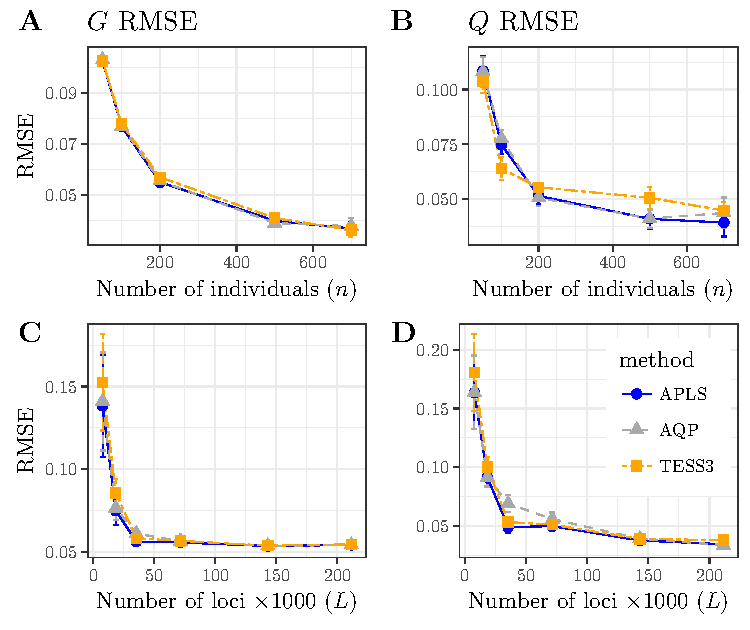
\includegraphics[width=\textwidth]{../Figure1/Figures/figure1.pdf}
\end{center}  
\noindent{\bf Figure 1.} {\bf Root Mean Squared Errors (RMSEs) for the $Q$ and $G$ matrix estimates.} Simulations of spatially admixed populations. A-B) Statistical errors for APLS, AQP and {\tt tess3} estimates as a function of the sample size, $n$ ($L \sim 10^4$). C-D) Statistical errors for APLS, AQP and {\tt tess3} estimates as a function of the number of loci, $L$ ($n = 200$).

\clearpage 
\newpage


\begin{center}
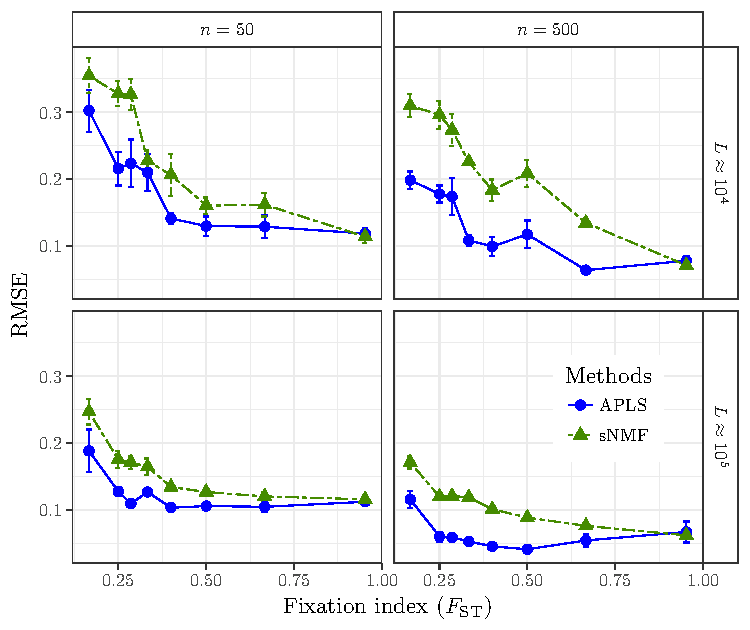
\includegraphics[width=\textwidth]{../Figure2/Figures/figure2.pdf}
\end{center}  
\noindent{\bf Figure 2.} {\bf Root Mean Squared Errors (RMSEs) for the $Q$ estimates.} Simulations of spatially admixed populations for several values of fixation index ($F_{\rm ST}$) between ancestral populations. Ancestral populations are simulated with Wright's two-island models and the fixation index is defined as $1 / (1 + 4 N_0 m)$ where $m$ is the migration rate and $N_0$ the effective population size. The statistical errors for sNMF and APLS are represented as a function of $F_{\rm ST}$. 

\clearpage 
\newpage

\begin{center}
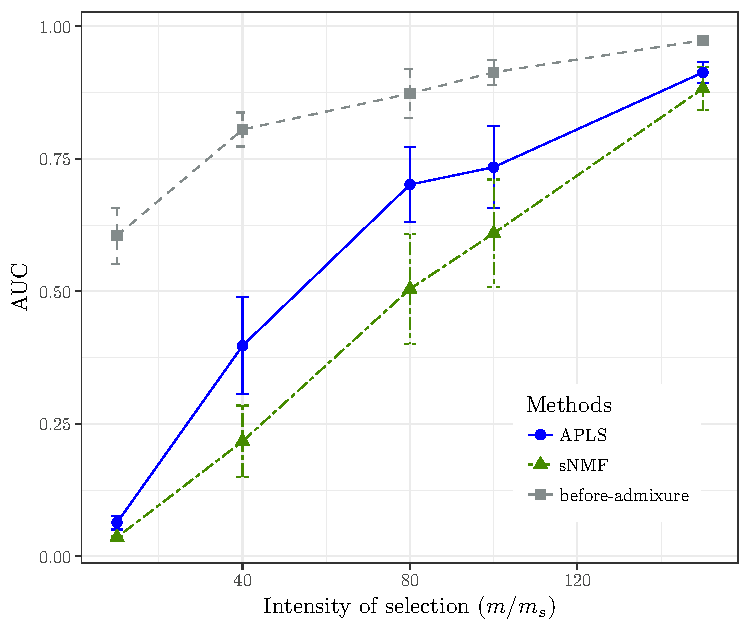
\includegraphics[width=\textwidth]{../Figure3/Figures/figure3.pdf}
\end{center}
\noindent{\bf Figure 3.} {\bf Area under the precision-recall curve (AUC)}. Neutrality tests applied to simulations of spatially admixed populations. AUCs for tests based on $F_{\rm ST}$ with the true ancestral populations,  spatial ancestry estimates computed with APLS algorithms, non-spatial ({\tt structure}-like) ancestry estimates computed with the {\tt snmf} algorithm. The relative intensity of selection in ancestral populations, defined as the ratio $m/m_s$, was varied in the range $1-160$.


\clearpage 
\newpage

\begin{center}
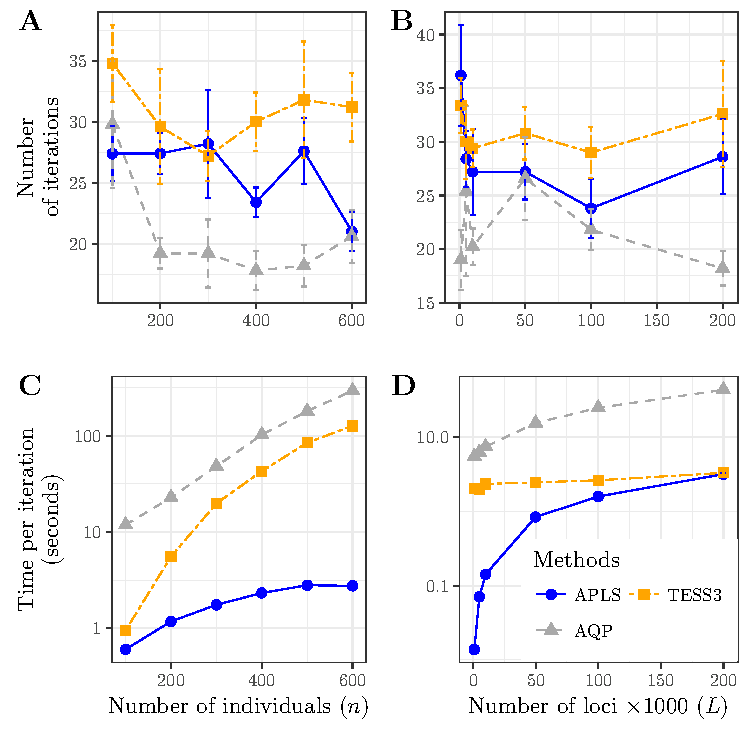
\includegraphics[width=\textwidth]{../Figure4/Figures/figure4.pdf}
\end{center}
\noindent{\bf Figure 4.} {\bf Number of iterations and runtimes for the AQP, APLS and {\tt tess3} algorithm implementations}. A-B)   Total number of iterations before an algorithm reached a steady solution. C-D) Runtime for a single iteration (seconds). The number of SNPs was kept fixed to $L = 50$k in A and C. The number of individuals was kept fixed to $n = 150$ in B and D.


\clearpage 
\newpage

\begin{center}
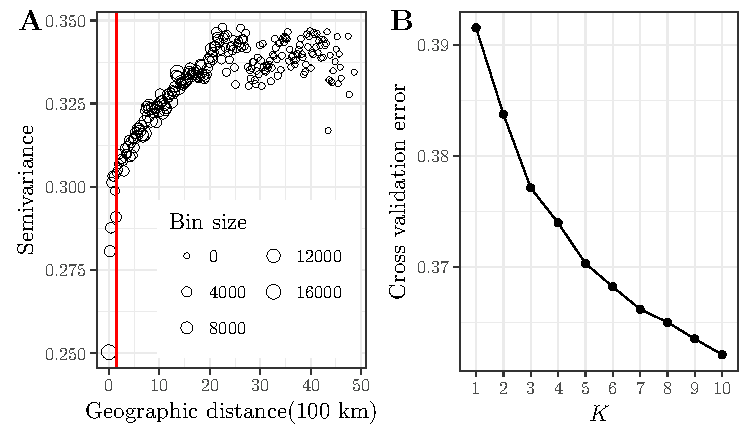
\includegraphics[width=\textwidth]{../Figure5/Figures/figure5.pdf}
\end{center}
\noindent{\bf Figure 5.} {\bf Range $\sigma$ and choice of $K$ for the APLS algorithm}. A) Empirical variogram for the {\it A. thaliana} data. The red vertical line shows the range value $\sigma = 1.5$. B) Cross validation error as function of the number of ancestral populations, $K$.

\clearpage 
\newpage

\begin{center}
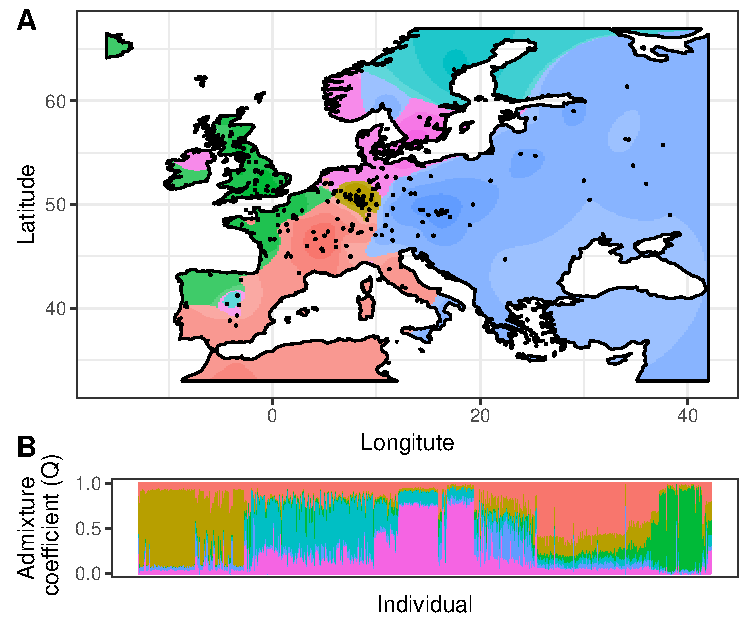
\includegraphics[width=\textwidth]{../Figure5/Figures/map.pdf}
\end{center}
\noindent{\bf Figure 6.} {\bf {\it A. thaliana} ancestry coeficients}. Ancestry coefficient estimates computed by the APLS algorithm with $K=6$ ancestral populations and $\sigma = 1.5$ for the range parameter. A) Geographic map of ancestry coefficients. B) Barplot of ancestry coefficients.

\clearpage 
\newpage

\begin{center}
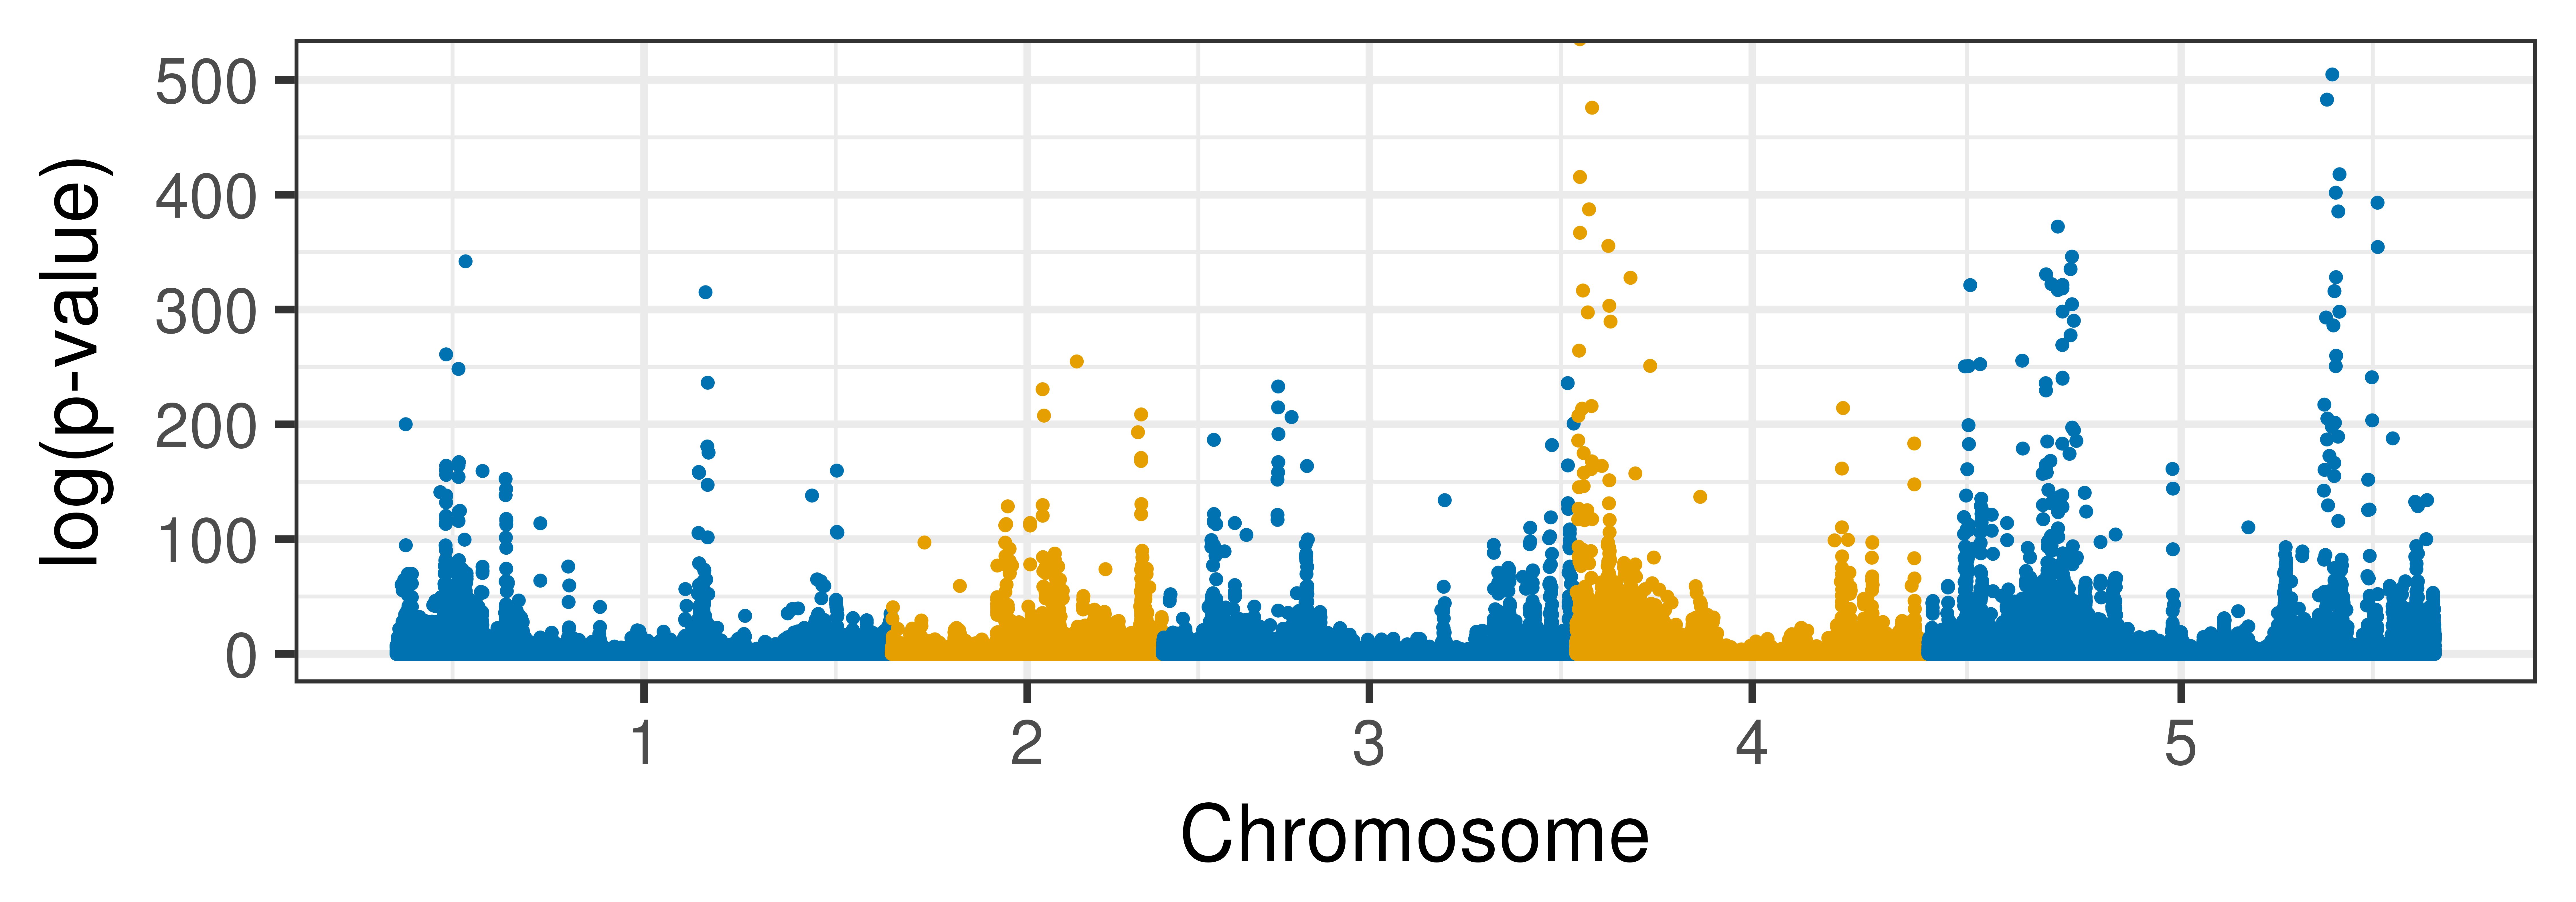
\includegraphics[width=0.60\paperwidth]{../Figure5/Figures/manhattanplot.png}
%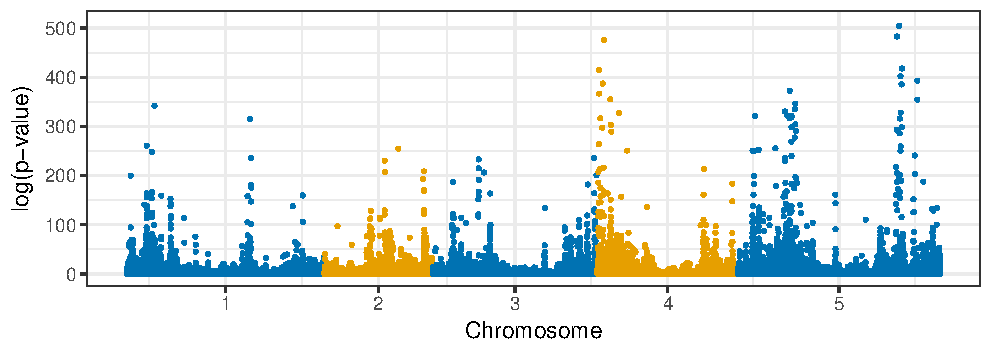
\includegraphics[width=\textwidth]{../Figure5/Figures/manhattanplot.pdf}
\end{center}
\noindent{\bf Figure 7.} {\bf Local adaptation in European lines of \bf {\it A.  thaliana} }. Manhattan plot of $-\log(p$\rm -value$)$.  $p$-value were computed from population structure estimated by the APLS algorithm with $K=6$ ancestral populations and $\sigma = 1.5$ for the range parameter.

%\includegraphics[width=12cm]{Figures/Figure_2.pdf}
%\noindent{\bf Figure 2.} {\bf .} 




\end{document}
